\documentclass{article}
\usepackage[utf8]{inputenc}
\usepackage[spanish,mexico]{babel}
\usepackage[margin=2.5cm]{geometry}
\usepackage{graphicx}
\usepackage[export]{adjustbox}
\usepackage{caption}
\usepackage{subcaption}
\usepackage{fancyhdr}
\usepackage{enumitem}
\usepackage{amsmath}
\usepackage{amssymb}
\usepackage{amsfonts}
\usepackage{booktabs}
\usepackage{hyperref}
\pagestyle{fancy}
\fancyhf{}

\title{Template Facultad de Ciencias, UNAM}
\author{Isidro Armando de Ojalvo Abelló García}
\date{\today}

\begin{document}

\thispagestyle{empty}

	\begin{figure}[ht]
	   \minipage{0.76\textwidth}
			
\includegraphics[width=4cm]{Logo_UNAM.png}
			\label{EscudoUNAM}
	   \endminipage
	   \minipage{0.32\textwidth}
			
\includegraphics[height=4.3cm ,width=4.3cm]{Logo_FC.png}
			\label{EscudoFC}
		\endminipage
	\end{figure}

	\begin{center}
	\vspace{0.8cm}
	\LARGE
	UNIVERSIDAD NACIONAL AUTÓNOMA DE MÉXICO

	\vspace{0.8cm}
	\LARGE
	FACULTAD DE CIENCIAS

	\vspace{1.7cm}
	\Large
	\textbf{REPORTE\\ Segundo Proyecto: OjalvoMusic}

	\vspace{1.3cm}
	\normalsize
	PRESENTA \\
	\vspace{.3cm}
	\large
	\textbf{Isidro Armando Abelló García \\ 426009038}

	\vspace{1.3cm}
	\normalsize
	PROFESOR \\
	\vspace{.3cm}
	\large
	\textbf{Dr. Canek Peláez Valdés}

	\vspace{1.3cm}
	\normalsize
	ASIGNATURA \\
	\vspace{.3cm}
	\large
	\textbf{Modelado y Programación}

	\vspace{1.3cm}
	\today
	\end{center}

	\newpage

\section{Introducción}

El proyecto consiste en una biblioteca musical de escritorio,
\texttt{ojalvomusic}. El enunciado pide cuatro componentes:

\begin{enumerate}
	\item Una \textbf{base de datos} SQLite con un esquema fijo
	(\texttt{rolas.sql}), que no se puede modificar.
	\item Un \textbf{minero} que recorre un directorio, lee las etiquetas
	ID3v2.4 de los archivos MP3 y guarda su información en la base de datos.
	\item Una \textbf{interfaz gráfica} para consultar y modificar esos
	datos: editar rolas y álbumes, definir intérpretes como personas o grupos
	y agregar personas a grupos.
	\item Una forma de \textbf{buscar} rolas por campos sin escribir SQL.
\end{enumerate}

Como punto extra se pide \textbf{reproducir} los MP3. Una regla atraviesa
todo el proyecto: los archivos MP3 nunca se modifican; cualquier cambio
ocurre solo en la base de datos.

Desde el principio decidí escribirlo en \textbf{C\#}, porque su orientación
a objetos lo hace ideal para un proyecto con tantas piezas que colaboran
entre sí. Quedaba elegir el entorno gráfico; después de investigar las
opciones disponibles escogí \textbf{Avalonia}, por ser multiplataforma.

Este reporte describe cómo se desarrolló el proyecto: la metodología que
seguí, los siete problemas en los que dividí el trabajo, las técnicas y
patrones de diseño que usé en cada uno, y lo que aprendí. El uso del programa
está en el README y en el manual de usuario (archivos \texttt{README.md} y
\texttt{MANUAL.md} del repositorio).

\section{Desarrollo}

\subsection{Metodología}

A partir de la experiencia de mi proyecto anterior, y después de analizar el
problema, decidí usar una metodología \textbf{ágil}, para ser más versátil al
abordar cada dificultad. Separé el problema principal en siete subproblemas
``grandes'' (tabla \ref{tab:problemas}) y a cada uno le apliqué un pequeño
esquema de \textbf{cascada}: análisis, diseño, desarrollo y pruebas.

\begin{table}[htbp]
	\centering
	\begin{tabular}{cll}
		\toprule
		\textbf{\#} & \textbf{Problema} & \textbf{Fechas (2026)} \\
		\midrule
		0 & Control y acceso a la base de datos & 16 de octubre \\
		1 & Minero & 18 al 23 de octubre \\
		2 & Controlador de entrada & 27 al 31 de octubre \\
		--- & Reestructuración de la solución & 1 de noviembre \\
		3 & Interfaz gráfica en Avalonia & 3 al 7 de noviembre \\
		4 & Buscador de rolas & 8 al 10 de noviembre \\
		5 & Personas y grupos & 10 y 11 de noviembre \\
		6 & Reproductor de música (punto extra) & 11 y 12 de noviembre \\
		\bottomrule
	\end{tabular}
	\caption{Problemas en los que se dividió el trabajo.}
	\label{tab:problemas}
\end{table}

En cada paso traté de aplicar \textbf{``code a little, test a little''}:
escribir un trozo pequeño de código y probarlo antes de seguir. El historial
lo refleja: son alrededor de 60 commits pequeños, cada uno con un solo
propósito, y el proyecto termina con 311 pruebas.

\subsection{Problema 0: control y acceso a la base de datos}

\textbf{Análisis.} Había que crear el acceso a la base de datos y permitir
su modificación. El esquema ya estaba dado y no se podía cambiar, así que el
trabajo era envolverlo bien. También había que decidir qué hace única a cada
cosa: una rola es su ruta, un álbum es su nombre más su directorio, y un
intérprete es su nombre exacto.

\textbf{Diseño.} El profesor Canek sugirió usar el patrón \textbf{DAO}
(\emph{Data Access Object}) y decidí hacerle caso. Cada tabla tiene un DAO
que encapsula su SQL detrás de una interfaz (\texttt{IRolaDao},
\texttt{IAlbumDao}, \texttt{IPerformerDao}), de modo que el resto del
programa no escribe consultas. Agregué además un manejador de transacciones,
\texttt{UnitOfWork}, para garantizar limpieza y seguridad al tocar la base:

\begin{itemize}
	\item Es dueño de una sola conexión y de la transacción en curso. Los
	DAOs reciben el \texttt{UnitOfWork}, no la conexión.
	\item Implementa \texttt{IDisposable}: al salir del bloque
	\texttt{using}, una transacción sin confirmar se deshace sola.
	\item Cada operación abre su propio \texttt{UnitOfWork}, así que una
	conexión nunca se comparte entre hilos.
\end{itemize}

\textbf{Desarrollo.} Comencé por los modelos y los DAOs de rolas, álbumes e
intérpretes, que es lo que llenaría el minero en el problema 1. La base se
crea a partir de \texttt{rolas.sql}, que viaja intacto como recurso embebido
(\texttt{DatabaseInitializer}). Todas las consultas usan parámetros; nunca se
concatena texto, lo que brinda seguridad contra ataques de inyección de SQL
(\emph{SQL injection}).

\textbf{Pruebas.} Decidí delegar las pruebas de esta parte hasta que el
minero estuviera listo, porque el minero es su primer usuario real. Con él
llegaron las pruebas del inicializador (creación, segunda llamada, esquemas
ajenos, bases corruptas, llaves foráneas) y más adelante las de cada DAO.

\textbf{Técnicas y patrones:} DAO, \emph{Unit of Work}, patrón
\emph{disposable}, programación contra interfaces, consultas parametrizadas,
transacciones.

\subsection{Problema 1: minero}

\textbf{Análisis.} El minero debe encontrar todos los MP3 de un directorio,
de forma recursiva; leer sus etiquetas sin modificarlos; inferir las rutas de
rolas y álbumes; y no duplicar lo que ya está en la base. Además no puede
congelar la interfaz mientras trabaja, y debe poder cancelarse.

\textbf{Diseño.} Subdividí el problema en varias clases, cada una con una
sola responsabilidad:

\begin{itemize}
	\item \texttt{FileScanner} obtiene los archivos.
	\item \texttt{TagReader} lee las etiquetas (con la biblioteca
	TagLibSharp, sobre una abstracción de archivo de solo lectura).
	\item \texttt{Miner} orquesta la minería e integra lo resuelto en el
	problema 0.
\end{itemize}

El minero trabaja en dos fases: primero lee las etiquetas y después guarda
todo en una transacción, de modo que si algo falla a la mitad, la base no
queda a medias. Una decisión importante fue comprobar si una rola ya existe
\textbf{consultando la base de datos}, en lugar de copiar las rutas a
memoria. Esto prioriza la memoria y la simplicidad del código sobre la
velocidad: se cambia una búsqueda $O(1)$ en una tabla hash por una
$O(\log n)$ en el índice de la base.

Garanticé además que la minería fuera segura con hilos. Corre fuera del hilo
de la interfaz (\texttt{Task.Run}), un semáforo (\texttt{SemaphoreSlim})
impide dos minerías simultáneas, el avance se reporta con \texttt{IProgress}
y la cancelación es cooperativa, con \texttt{CancellationToken}.

\textbf{Desarrollo.} Primero hice una ``maqueta'' del minero, sin probar,
junto con el inicializador de la base y los contratos (interfaces y objetos
de transferencia como \texttt{TagInfo} y \texttt{MiningResult}). En ese paso
corregí también el error de la primera versión, que sacaba prácticamente toda
la base para hacer comprobaciones en C\#.

\textbf{Pruebas.} Fue el bloque de pruebas más grande del proyecto. El
minero recibe sus piezas por \textbf{inyección de dependencias}, y eso
permitió usar técnicas de \emph{mocking}: en las pruebas se le entregan
dobles (\texttt{FakeFileScanner}, \texttt{FakeTagReader}) en lugar de las
piezas reales. Se probaron el minado normal, la segunda corrida,
cancelaciones, archivos corruptos, duplicados y el minado simultáneo. Una
prueba de integración junta las tres piezas reales sobre un conjunto de MP3
generados (\texttt{Dataset/}), y otra comprueba que los MP3 no se modifican.

\textbf{Técnicas y patrones:} responsabilidad única, inyección de
dependencias por constructor, dobles de prueba, DTOs, tareas asíncronas,
semáforos, cancelación cooperativa.

\subsection{Problema 2: controlador de entrada}

\textbf{Análisis.} El programa se invoca como
\texttt{ojalvomusic [opciones] [ruta]} y, según los parámetros, debe minar,
abrir la interfaz, hacer ambas cosas o mostrar la ayuda. Los errores de uso
deben reportarse de forma limpia y con un código de salida.

\textbf{Diseño.} Para seguir el patrón \textbf{MVC} creé un
\texttt{Controller} que orquesta lo que hace el programa según la entrada. El
análisis de los parámetros quedó aparte, en \texttt{ArgumentParser}: una
función pura que recibe los argumentos y regresa las opciones, o lanza una
\texttt{UsageException}. Implementé también una \textbf{bitácora} para tener
mejor control del flujo del programa. Es una interfaz (\texttt{ILog}) con dos
implementaciones: \texttt{ConsoleLog}, que se activa con \texttt{-l}, y
\texttt{NullLog}, que aplica el patrón \emph{Null Object} para no llenar el
código de comprobaciones.

El controlador también usa inyección de dependencias: recibe los flujos de
salida, una función que fabrica el minero y una acción que abre la vista. Así
no conoce la interfaz gráfica y puede probarse sin ella.

\textbf{Desarrollo.} Se hizo en este orden: punto de entrada, parser de
argumentos, controlador y bitácora. Los códigos de salida siguen las
convenciones: 0 éxito, 1 error, 2 uso inválido y 130 cancelado con Ctrl+C.

\textbf{Pruebas.} Cada pieza tiene las suyas. Las del parser cubren cada
opción y cada error de uso. Las del controlador le inyectan un
\texttt{StringWriter} y un minero armado con piezas falsas, y revisan
mensajes y códigos de salida.

\textbf{Técnicas y patrones:} MVC, \emph{Null Object}, inyección de
dependencias con delegados (\texttt{Func}, \texttt{Action}), funciones puras,
excepciones propias.

\subsection{Reestructuración de la solución}

Mi idea original era tener un solo proyecto. Cuando estaba integrando
Avalonia me di cuenta de que eso sería problemático: sus paquetes podían
``contaminar'' el proyecto, de modo que para correr pruebas o ejecutar solo
cosas del modelo se iba a cargar la interfaz. Además todo quedaría
desorganizado, e incluso podría violarse la separación de responsabilidades.

Opté entonces por una solución con \textbf{tres proyectos}:

\begin{verbatim}
    MusicLib/         el modelo, como biblioteca
    MusicLib.UI/      el punto de entrada y la interfaz
    MusicLib.Tests/   las pruebas
\end{verbatim}

Las dependencias van en un solo sentido: la interfaz y las pruebas conocen al
modelo, pero el modelo no conoce a ninguna de las dos.

\subsection{Problema 3: interfaz gráfica en Avalonia}

\textbf{Análisis.} Aquí el problema era, sobre todo, aprender: los básicos
de Avalonia, su lenguaje de marcado (XAML) y la forma en que una ventana se
comunica con el código.

\textbf{Diseño.} Decidí aplicar, con perspectivas a futuro, el patrón
\textbf{Modelo-Vista-VistaModelo (MVVM)} en lugar de MVC, porque Avalonia
cuenta con una herramienta (Community Toolkit) que hace más fácil y natural
usarlo. En este patrón, el VistaModelo se encarga más activamente de
controlar el estado de su ventana que de comunicarse con el modelo, pero
cumple los mismos objetivos de separación de responsabilidades y organización
que MVC. Como me dijo el profesor Canek: ``(\ldots) MVVM es MVC con pasos
extra (\ldots)''.

La vista se enlaza al VistaModelo con \emph{bindings}: cuando una propiedad
cambia, la ventana se actualiza sola, y los botones ejecutan comandos del
VistaModelo. Para lo que el VistaModelo no debe hacer directamente, definí
servicios que se le inyectan: uno para elegir carpetas y una clase auxiliar
para abrir ventanas modales, pensada para los problemas siguientes.

\textbf{Desarrollo.} Primero hice maquetas, solo visuales, de las ventanas
que iba a usar: la principal, la búsqueda avanzada, los formularios y el
editor. Después conecté la primera funcionalidad real, el ciclo de vida del
botón Minar: elegir la carpeta, mostrar el avance, cancelar y cargar las
rolas en la tabla.

\textbf{Pruebas.} La interfaz se verificó a mano, ventana por ventana. El
modelo siguió cubierto por sus pruebas automáticas, que no cargan Avalonia
gracias a la reestructuración.

\textbf{Técnicas y patrones:} MVVM, \emph{Observer} (notificación de cambios
y eventos), \emph{Command}, enlace de datos, servicios inyectados.

\subsection{Problema 4: buscador de rolas}

\textbf{Análisis.} El problema se dividió en dos: la búsqueda general, con
un solo texto que se busca en título, intérprete, álbum y género; y la
búsqueda avanzada, por campos separados y rango de años. El usuario nunca
escribe SQL.

\textbf{Diseño.} La infraestructura ya estaba hecha, así que solo hubo que
extender los DAOs para que hicieran consultas no triviales, con
\texttt{JOIN} entre rolas, intérpretes y álbumes. Los criterios viajan en un
objeto (\texttt{RolaSearch}), y una clase pequeña (\texttt{RolaSearchSql})
arma la consulta agregando una condición fija por cada criterio con valor,
siempre con parámetros. Para que la búsqueda no distinga mayúsculas ni
acentos, un normalizador de texto se registra como función dentro de SQLite,
sin tocar el esquema.

\textbf{Desarrollo.} Primero el DAO, después la búsqueda general conectada a
la vista y por último la ventana de búsqueda avanzada con su VistaModelo. En
la vista bastó acomodar los \emph{bindings}. La granularidad y la separación
entre Modelo, Vista y VistaModelo resultaron muy convenientes: cada cambio
tocó pocas piezas.

Con la tabla ya funcionando agregué sobre la misma base la \textbf{edición
de rolas y álbumes}: el \texttt{UPDATE} en los DAOs, una clase del modelo
(\texttt{LibraryEditor}) que valida y guarda cada cambio en una transacción,
los editores en la interfaz y la portada de la rola seleccionada.

\textbf{Pruebas.} Se probaron el normalizador, el armado del SQL y el DAO;
el resto de la búsqueda se verificó en la vista. El editor tiene pruebas
propias para cada regla.

\textbf{Técnicas y patrones:} objeto de criterios, consultas parametrizadas
armadas dinámicamente, función SQL definida por el programa, capa de servicio
con una transacción por operación, \emph{bindings}.

\subsection{Problema 5: personas y grupos}

\textbf{Análisis.} El manejo de este problema se parece mucho al anterior.
Lo separé en dos: el de las personas y el de los grupos. Para cada uno
elaboré una serie de reglas, que están especificadas en el manual. Por
ejemplo: qué pasa al agregar una persona cuyo nombre ya es un intérprete, qué
se borra al eliminar un grupo, y cómo se validan las fechas.

\textbf{Diseño.} Extendí los DAOs (\texttt{PersonDao}, \texttt{GroupDao} y
\texttt{MembershipDao} para la tabla \texttt{in\_group}) y agregué dos
editores en el modelo, \texttt{PersonsEditor} y \texttt{GroupsEditor}. Cada
operación valida y cambia la base en una sola transacción. Las reglas de
validación viven en el modelo y los VistaModelos las reutilizan: el botón
Guardar se deshabilita mientras los datos sean inválidos, y la ventana dice
el motivo.

\textbf{Desarrollo.} Escribí un plan de 17 pasos, un commit por paso:
primero el modelo y después la interfaz. Esta última incluye las ventanas de
lista, un mismo formulario para agregar y editar, un diálogo genérico de
confirmación antes de borrar y una lista doble para elegir a los miembros de
un grupo.

\textbf{Pruebas.} Cada DAO y cada editor llegaron con sus pruebas, que
cubren conflictos de nombres, fechas inválidas, borrados y membresías. La
interfaz se verificó a mano.

\textbf{Técnicas y patrones:} DAO, capa de servicio, transacciones,
validación compartida entre modelo y VistaModelo, comandos con condición de
ejecución, reutilización de ventanas.

\subsection{Problema 6: reproductor de música}

\textbf{Análisis.} Avalonia no reproduce audio, así que el punto extra se
redujo prácticamente al uso de una biblioteca. Aun así hubo problemas no
triviales, relacionados con los hilos de ejecución, al implementar la barra
de progreso y lograr que sonara adecuadamente.

\textbf{Diseño.} Elegí LibVLCSharp, que usa el VLC instalado en el sistema.
El reproductor queda detrás de una interfaz (\texttt{IAudioPlayer}), con una
implementación que adapta la biblioteca (\texttt{VlcAudioPlayer}) y un
VistaModelo propio. Si VLC no está instalado, el programa no se cae: el
reproductor queda deshabilitado y lo avisa.

El problema de los hilos es que VLC avisa desde un hilo suyo, y la interfaz
solo puede tocarse desde el suyo. Lo resolví de dos formas:

\begin{itemize}
	\item El aviso de ``terminó la rola'' se pasa al hilo de la interfaz
	antes de atenderlo.
	\item La barra de progreso no escucha a VLC; un temporizador del hilo de
	la interfaz le pregunta la posición varias veces por segundo.
\end{itemize}

\textbf{Desarrollo.} En dos pasos: primero reproducir y pausar la rola
seleccionada, y después la barra de progreso con el tiempo y el salto a
cualquier punto.

\textbf{Pruebas.} No hay pruebas automáticas de audio; se verificó a mano:
reproducir, pausar, reanudar, cambiar de rola, llegar al final, saltar con la
barra y abrir el programa sin VLC.

\textbf{Técnicas y patrones:} \emph{Adapter}, inyección de dependencias,
eventos, paso de mensajes al hilo de la interfaz, temporizador de sondeo.

\section{Diagramas UML simplificados del proyecto}

Esta sección resume el diseño en tres diagramas de clases, uno por cada capa
del programa. Están simplificados a propósito: cada clase muestra solo sus
miembros principales, sin tipos ni parámetros, y se omiten las clases
auxiliares.

La figura \ref{fig:uml-datos} muestra los modelos y el acceso a la base de
datos. El \texttt{UnitOfWork} es dueño de la conexión y de los seis DAOs, y
los tres editores lo usan para cambiar la base en una sola transacción.

\begin{figure}[htbp]
	\centering
	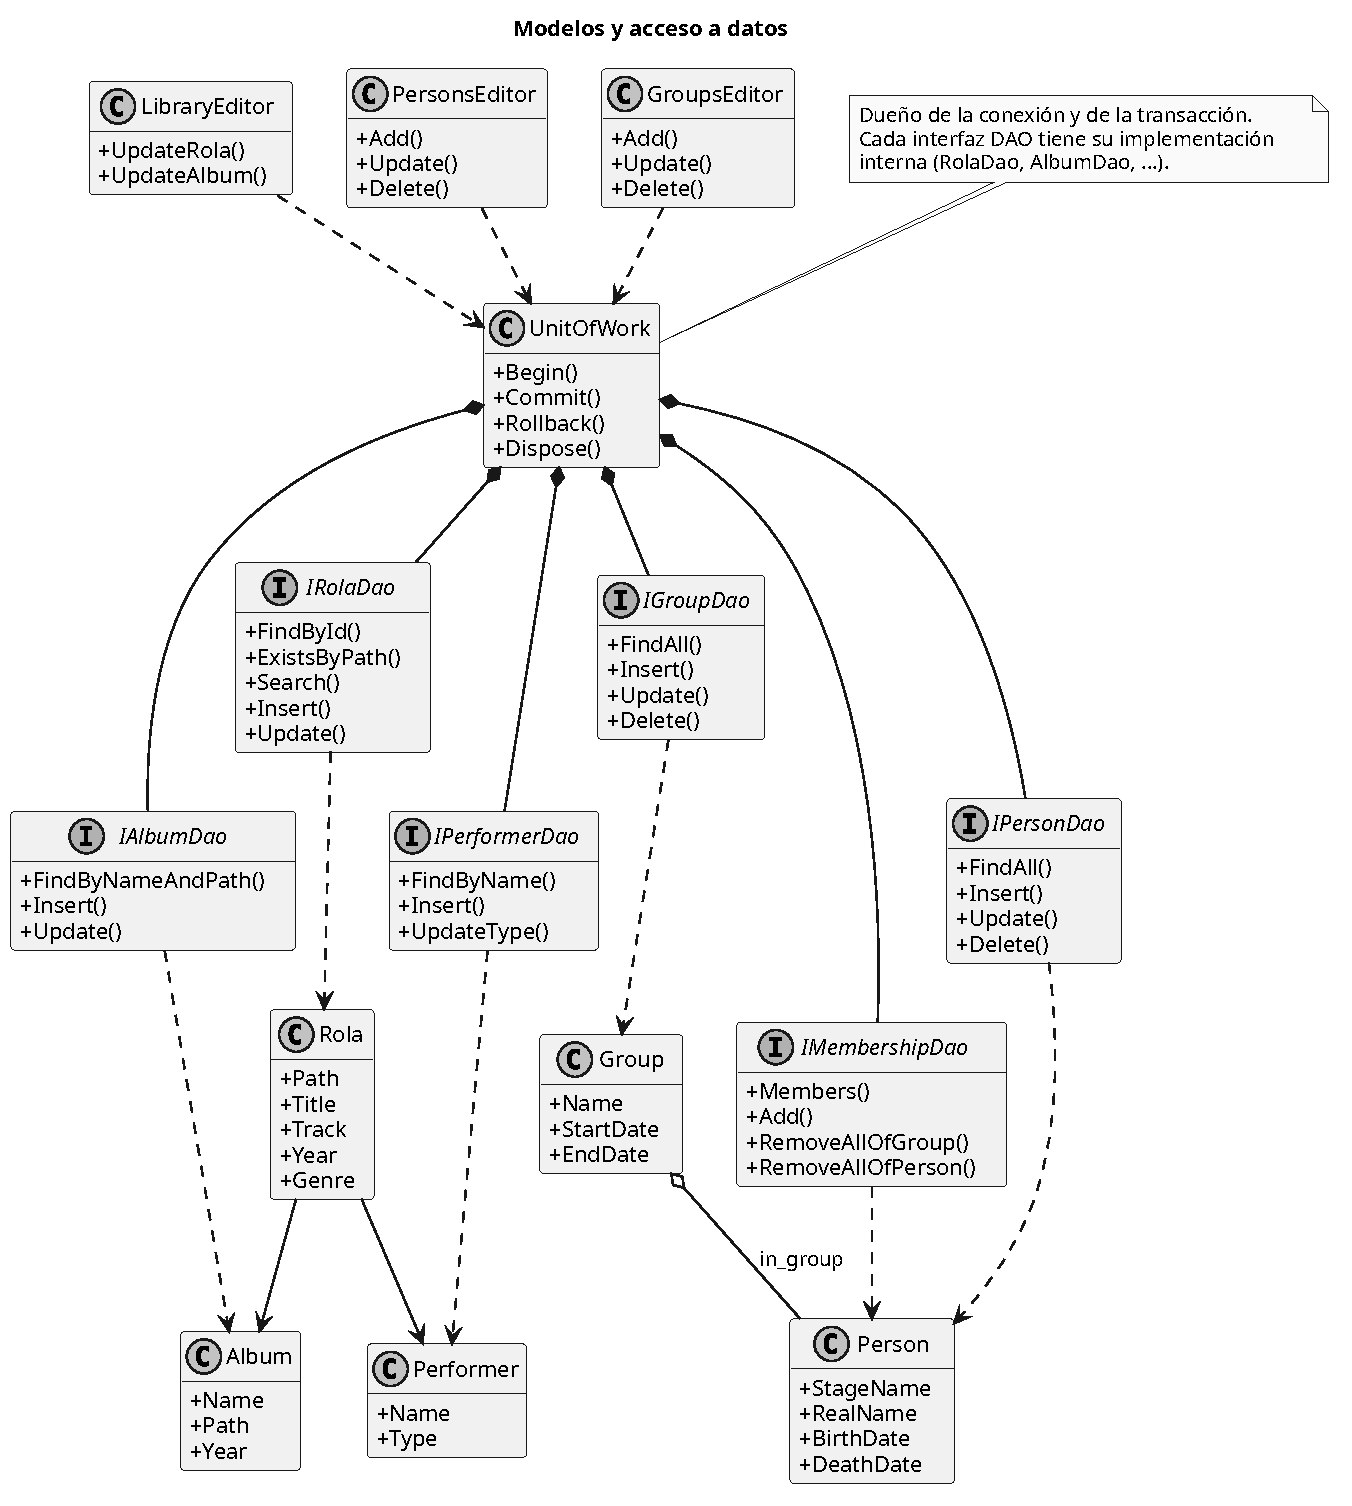
\includegraphics[width=\linewidth,height=0.65\textheight,keepaspectratio]{AccesoDatosModelo.pdf}
	\caption{Modelos y acceso a datos (patrones DAO y \emph{Unit of Work}).}
	\label{fig:uml-datos}
\end{figure}

\newpage

La figura \ref{fig:uml-minero} muestra el camino desde el punto de entrada:
el \texttt{Controller} depura los parámetros, crea el minero y le entrega la
bitácora. El minero solo conoce las interfaces de sus piezas, lo que permite
sustituirlas en las pruebas.

\begin{figure}[htbp]
	\centering
	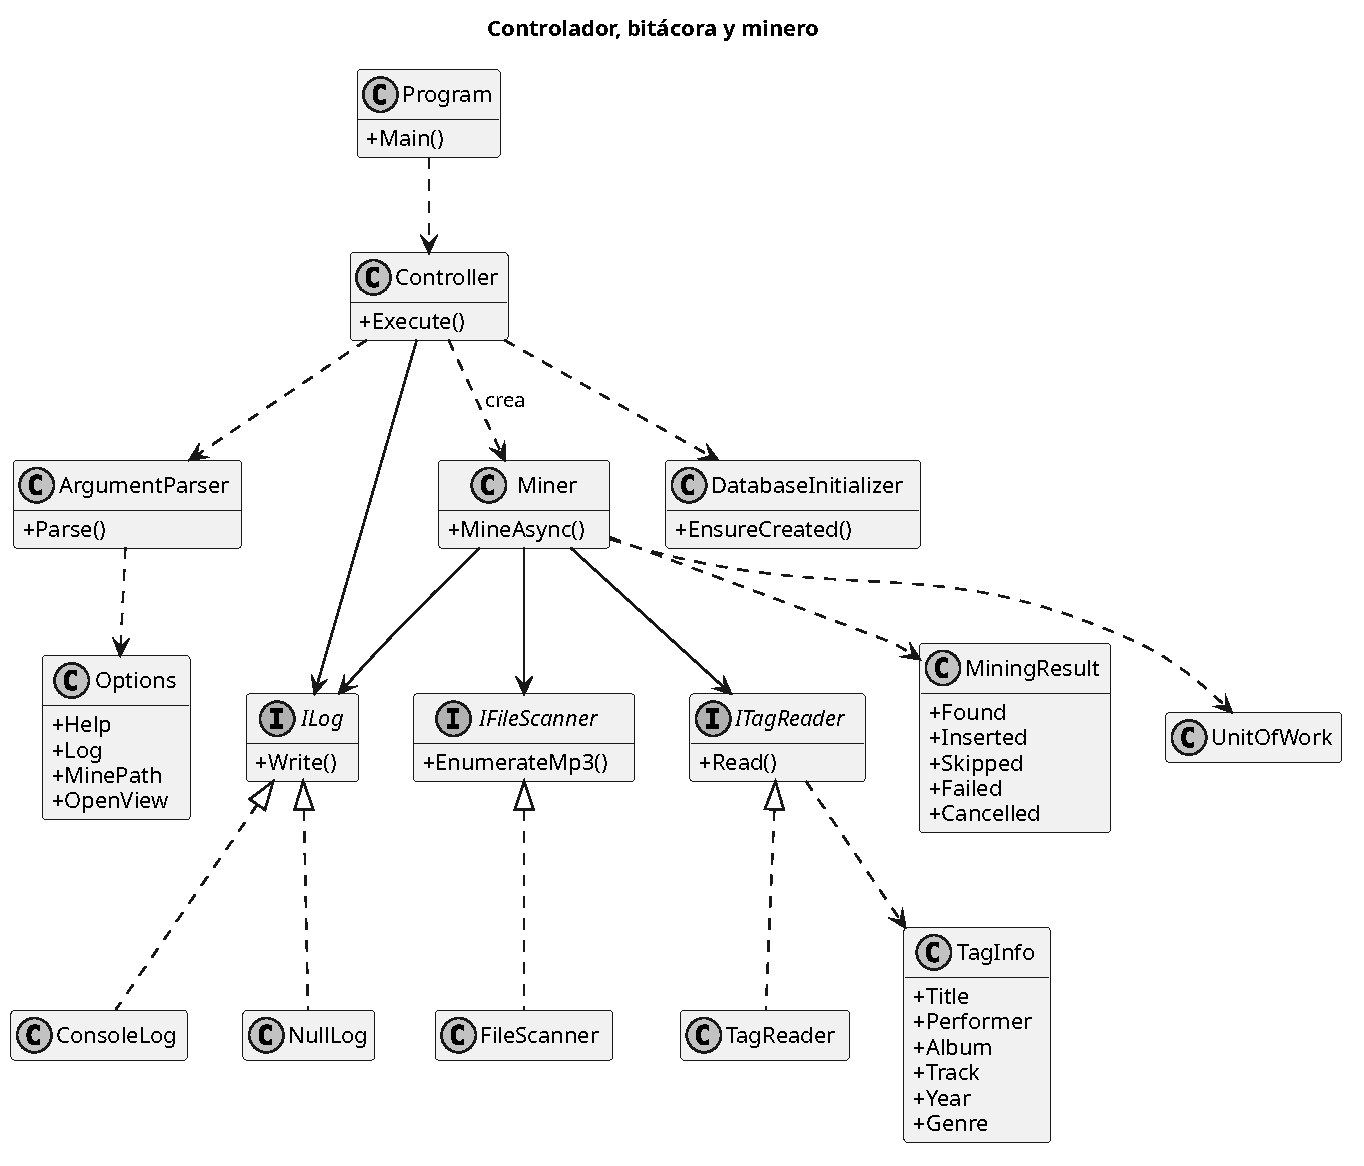
\includegraphics[width=\linewidth,height=.8\textheight,keepaspectratio]{ControladorBitacoraMinero.pdf}
	\caption{Controlador, bitácora y minero.}
	\label{fig:uml-minero}
\end{figure}

\newpage

La figura \ref{fig:uml-interfaz} muestra la interfaz gráfica. El VistaModelo
principal recibe sus servicios por inyección, y el servicio de diálogos crea
los VistaModelos de las ventanas secundarias, que a su vez usan los editores
del modelo. Las ventanas no se dibujan una por una: cada VistaModelo tiene la
suya.

\begin{figure}[htbp]
	\centering
	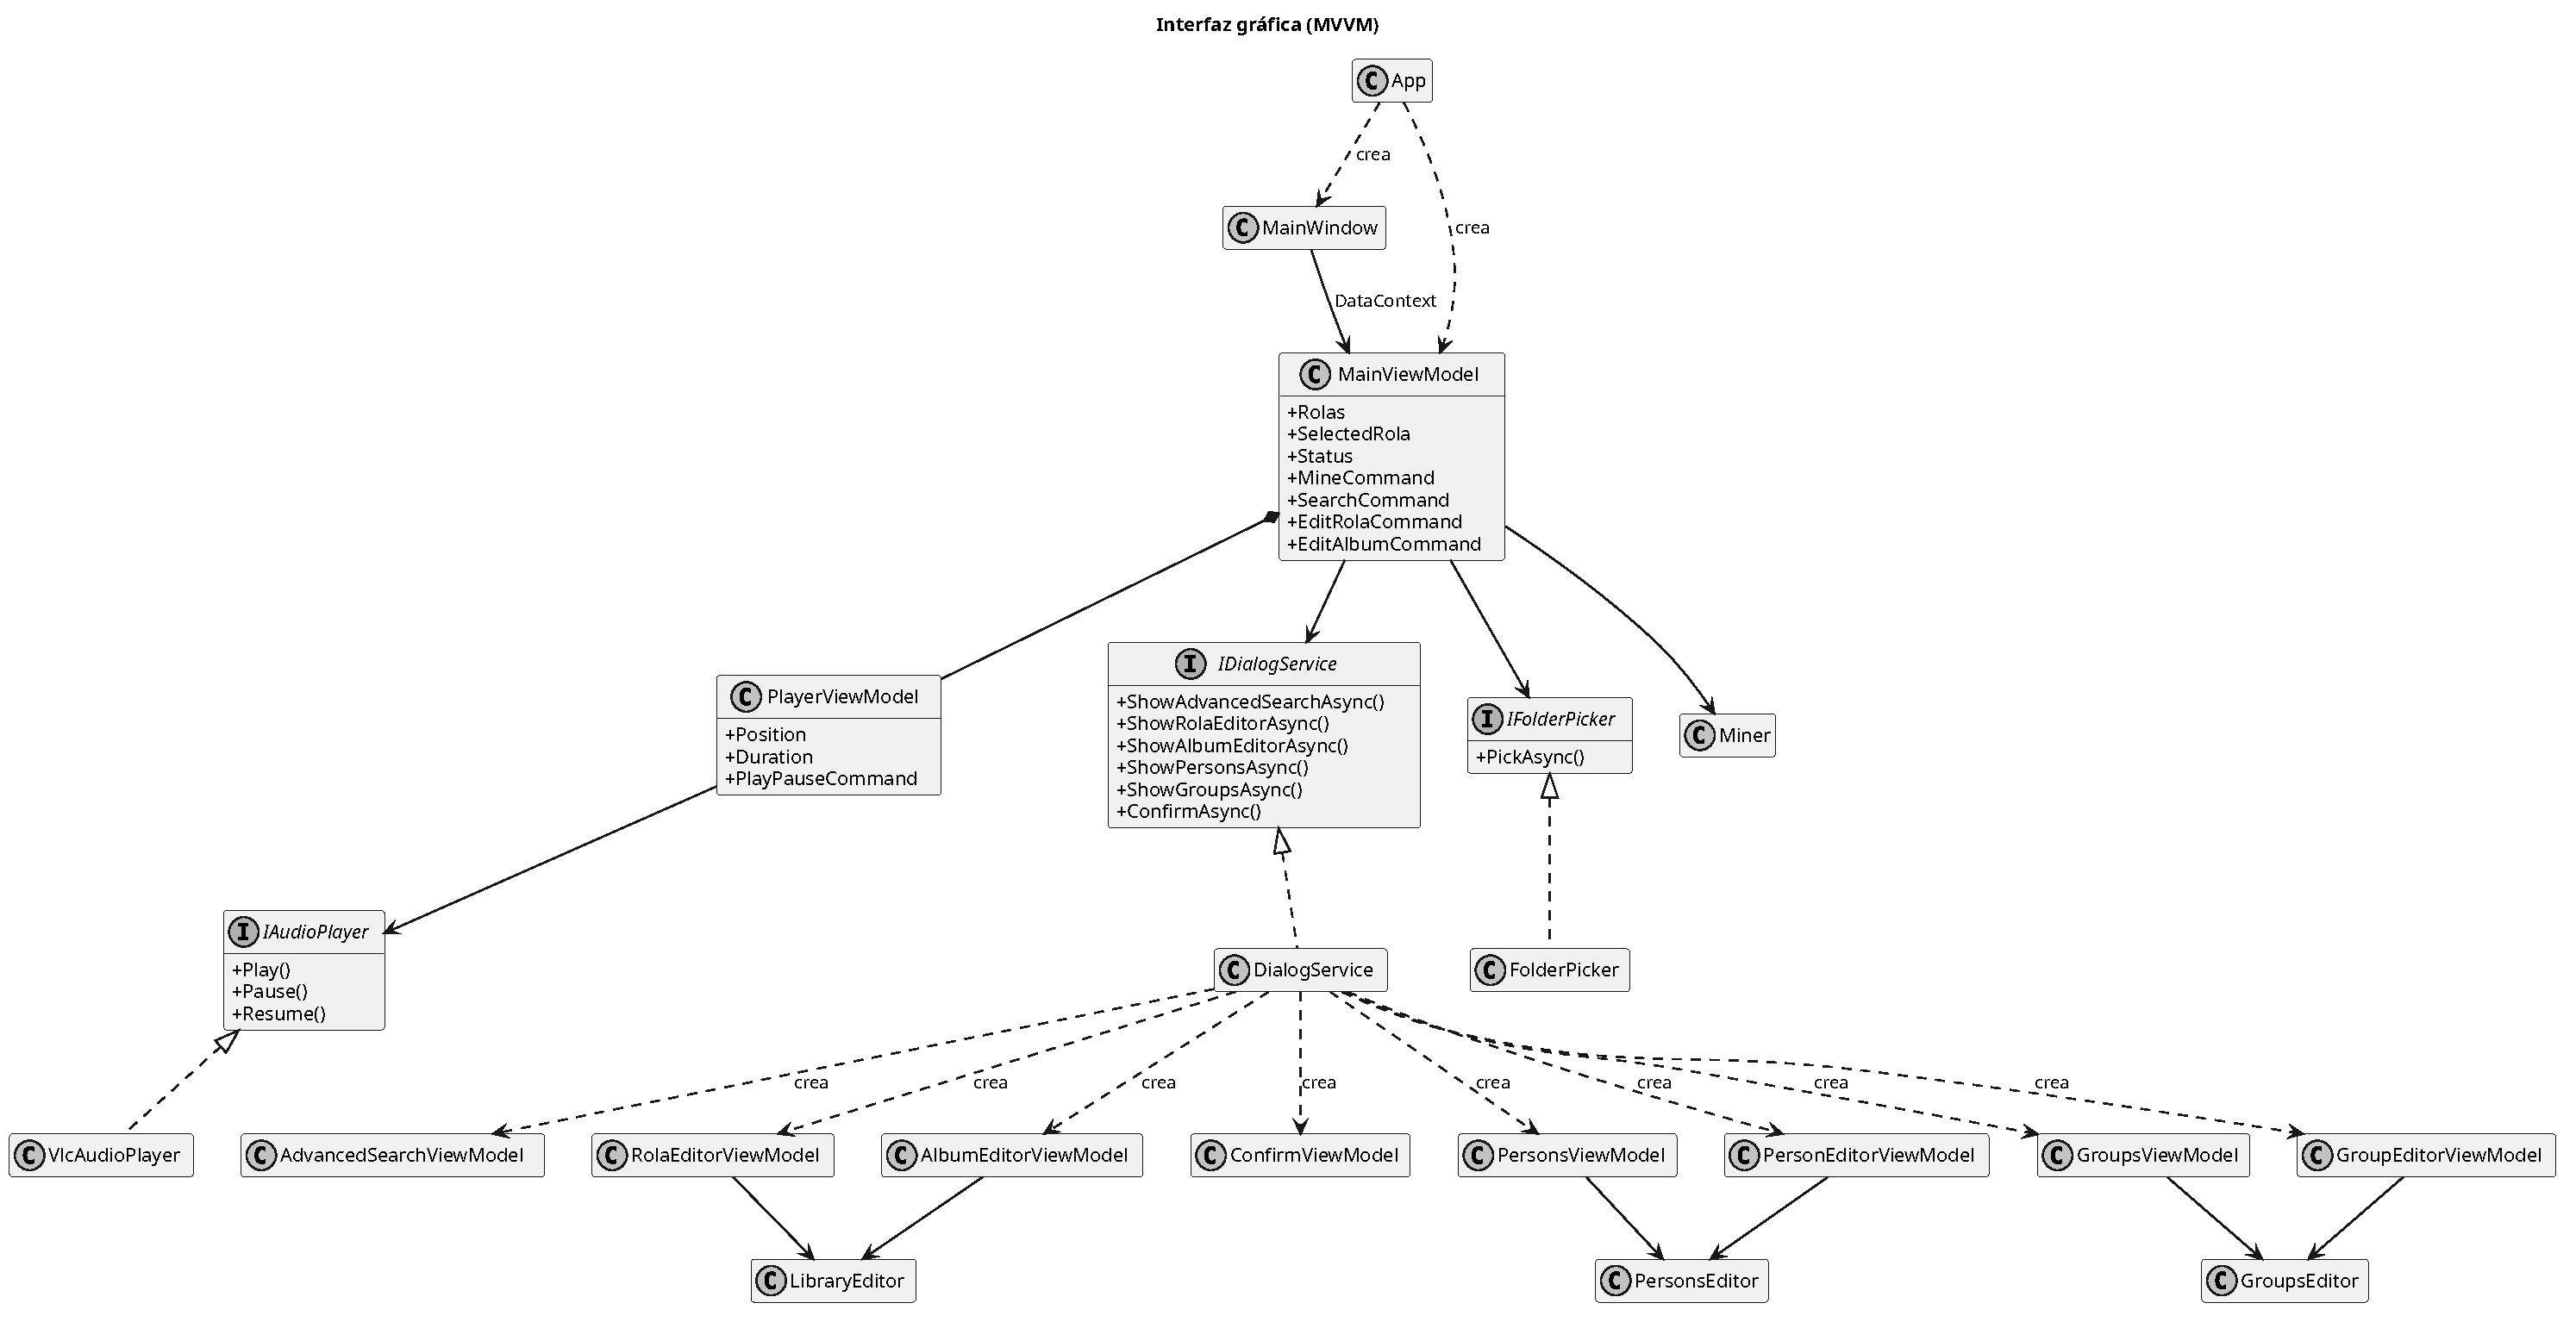
\includegraphics[angle=90,height=0.725\textheight,width=\linewidth,keepaspectratio]{MVVM.pdf}
	\caption{Interfaz gráfica (patrón MVVM). El diagrama está girado para
	aprovechar la página.}
	\label{fig:uml-interfaz}
\end{figure}

\newpage

\section{Conclusiones}

El proyecto fue muy importante para mi formación. Me obligó a pensar en el
diseño antes que en el código, y cada problema posterior resultó más fácil
gracias a las decisiones tomadas en los anteriores: para la búsqueda y para
las personas y grupos, la infraestructura ya estaba hecha, por ejemplo.

Aprendí patrones y técnicas nuevas:

\begin{itemize}
	\item \textbf{Bases de datos:} el patrón DAO, el lenguaje SQL (en
	particular con SQLite) y el manejo de transacciones.
	\item \textbf{C\#:} interfaces y bibliotecas útiles del lenguaje,
	delegados y eventos, el manejo de tipos anulables, el patrón
	\emph{disposable} y sus herramientas de pruebas.
	\item \textbf{Concurrencia:} hilos, tareas (\texttt{Task}), promesas y
	semáforos.
	\item \textbf{Pruebas:} inyección de dependencias y \emph{mocking}.
	\item \textbf{Interfaz gráfica:} Avalonia, el patrón MVVM y Community
	Toolkit.
\end{itemize}

Sobre la metodología, dividir el trabajo en problemas ``grandes'' y aplicar a
cada uno una pequeña cascada funcionó bien: siempre supe qué estaba
resolviendo y pude cambiar de rumbo cuando hizo falta, como en la
reestructuración de la solución.

Me hubiera gustado implementar un mejor buscador, en el que las personas y
los grupos se asociaran a las búsquedas de rolas. También me hubiera gustado
hacer un diseño más creativo de la interfaz, para darle un toque de
originalidad. Aun así, estoy muy conforme con el diseño general del programa.

\renewcommand{\refname}{Bibliografía}

\begin{thebibliography}{99}

	\bibitem{dao}
	Wikipedia. \emph{Data access object}.
	\url{https://en.wikipedia.org/wiki/Data_access_object}

	\bibitem{unitofwork}
	NetMentor. \emph{Unit of work pattern C\#}.
	\url{https://www.netmentor.es/entrada/en/unit-of-work}

	\bibitem{sqlite}
	SQLite. \emph{Sitio oficial y documentación}.
	\url{https://www.sqlite.org/}

	\bibitem{mssqlite}
	Microsoft. \emph{Microsoft.Data.Sqlite overview}. Microsoft Learn.
	\url{https://learn.microsoft.com/dotnet/standard/data/sqlite}

	\bibitem{taglib}
	Mono Project. \emph{TagLib\#} (taglib-sharp). GitHub.
	\url{https://github.com/mono/taglib-sharp}

	\bibitem{async}
	Microsoft. \emph{Asynchronous programming with async and await}.
	Microsoft Learn.
	\url{https://learn.microsoft.com/en-us/dotnet/csharp/asynchronous-programming/}

	\bibitem{xunit}
	xUnit.net. \emph{Sitio oficial y documentación}.
	\url{https://xunit.net/}

	\bibitem{mocking}
	Microsoft. \emph{Mocking for tests in C\#}. Code-With-Engineering
	Playbook.
	\url{https://microsoft.github.io/code-with-engineering-playbook/automated-testing/unit-testing/mocking/}

	\bibitem{nullobject}
	Refactoring.Guru. \emph{Introduce Null Object}.
	\url{https://refactoring.guru/introduce-null-object}

	\bibitem{mvc}
	Wikipedia. \emph{Model--view--controller}.
	\url{https://en.wikipedia.org/wiki/Model-view-controller}

	\bibitem{avalonia}
	Avalonia. \emph{Avalonia Docs}.
	\url{https://docs.avaloniaui.net/}

	\bibitem{mvvmwiki}
	Wikipedia. \emph{Model--view--viewmodel}.
	\url{https://en.wikipedia.org/wiki/Model-view-viewmodel}

	\bibitem{mvvm}
	Avalonia. \emph{The MVVM pattern}. Avalonia Docs.
	\url{https://docs.avaloniaui.net/docs/fundamentals/the-mvvm-pattern}

	\bibitem{toolkit}
	Microsoft. \emph{Introduction to the MVVM Toolkit}. Microsoft Learn.
	\url{https://learn.microsoft.com/en-us/dotnet/communitytoolkit/mvvm/}

	\bibitem{libvlcsharp}
	VideoLAN. \emph{LibVLCSharp}. GitHub.
	\url{https://github.com/videolan/libvlcsharp}

	\bibitem{jovanovic}
	Jovanovi\'c, M. \emph{Milan Jovanovi\'c} (canal de YouTube sobre
	arquitectura y patrones en .NET).
	\url{https://www.youtube.com/@MilanJovanovicTech}

\end{thebibliography}

\noindent Todas las fuentes se consultaron entre octubre y noviembre de 2026.

\end{document}